%----------------------------------------------------------------------------------------
%	CHAPTER ONE
%----------------------------------------------------------------------------------------

\chapter{Introduction to Deep Learning}
Deep learning is rooted in the concept of artificial neural networks (ANNs), which are computing systems inspired by the biological neural networks of the human brain. The basic idea dates back to the 1940s and 1950s when researchers began exploring the mathematical models of neurons. Yann LeCun's work in the 1980s, particularly his development of convolutional neural networks (CNNs)  \cite{lecun1989}, played a crucial role in advancing neural network research. However, despite these advancements, neural network research faced challenges, including limited computational power and insufficient data, leading to a period of stagnation during the 1970s and 1980s.

The breakthroughs that led to the modern era of deep learning began around the mid-2000s. The term ``deep learning" gained widespread recognition around 2012 when deep neural networks, particularly convolutional neural networks (CNNs)  \cite{krizhevsky2012ImageNet}, achieved ground-breaking performance in computer vision tasks, such as image classification, through competitions like the ImageNet Large Scale Visual Recognition Challenge (ILSVRC) \cite{web:ILSVRC}.

\section{Mathematics for Deep Learning}
It is crucial to have mathematical fundamentals to fully comprehend deep learning concepts. This section offers an overview of essential mathematical topics necessary for delving into deep learning algorithms. To fully grasp the content of this book on deep learning, it is essential for students to have a basic understanding of the following mathematical topics:

\begin{itemize}
  \item \textbf{Linear Algebra}: Linear algebra forms the foundation of many deep learning techniques. Concepts such as vectors, matrices, matrix operations (addition, multiplication), matrix factorization (e.g., Singular Value Decomposition), and eigenvalues/eigenvectors are important.
  \item \textbf{Calculus}: Calculus plays a vital role in understanding optimization algorithms used in training deep learning models. Concepts like derivatives, gradients, chain rule, optimization techniques (e.g., gradient descent, stochastic gradient descent), and convex optimization are essential.
  \item \textbf{Probability and Statistics}: Probability theory is important for understanding the uncertainty associated with data and predictions in deep learning models. Concepts like probability distributions (e.g., Gaussian distribution), expected value, variance, covariance, conditional probability, Bayes' theorem, and statistical inference are crucial.
  \item \textbf{Graph Theory}: Graph theory is relevant for understanding neural network architectures and operations. Concepts like directed and undirected graphs, nodes, edges, adjacency matrices, and graph algorithms (e.g., breadth-first search, depth-first search) are important for understanding the structure and behavior of neural networks.
\end{itemize}

\section{Artificial Neural Networks}

\subsection{Feedforward Neural Networks}
These are the simplest form of neural networks, consisting of an input layer, one or more hidden layers, and an output layer. Each neuron in one layer is connected to every neuron in the next layer, with no feedback connections.

\section{Different Deep Learning Algorithms}

Deep learning algorithms typically involve neural networks with multiple layers (hence the term "deep"), allowing them to automatically discover intricate patterns and representations from raw data. This section introduces some common types of deep learning algorithms:

\subsection{Convolutional Neural Network}
The example of "teaching a child to speak their first word" illustrates a supervised machine learning problem. This type of machine learning requires a pre-existing data-set with known information and desired outcomes. The machine learning model must learn from this dataset in order to predict the desired outcome.

Supervised machine learning is widely used in today's technologies across various fields such as bio-security, weather forecasting, text prediction, and spam detection, etc. These methods use pre-existing data that includes both input features and the desired output (or target variable) to understand the underlying relationship. The model learns from the data, and the resulting parameters can be used to predict outcomes for new data.

An example of supervised learning is a biometric authentication system that uses facial recognition or fingerprints for logging into computers or mobile phones. The system is trained to recognize an individual's unique bio-data through registration. Once registered, the system compares presented bio-data to the registered information, and grants ("accept") or denies access ("reject") accordingly. Another example is a weather forecasting system that provides numerical data as output.

Depending on the type of output, supervised learning methods can be divided into two categories: \textbf{classification}, which assigns a class label to new data (such as "accept" or "reject") and \textbf{regression}, which predicts a numerical value (such as weather data).

\subsection{Recurrent Neural Network}
Unsupervised machine learning refers to the process of analyzing data without a pre-existing labeled dataset. In this case, the machine learning method extracts information from the data on its own.

For example, imagine you are an active user of a social media page and your team has been uploading photos regularly for over a decade. One day, you decide to download all the photos and sort them based on similar activities. Manually checking and labeling each photo would be time-consuming as there are more than 100,000 photos. Unsupervised machine learning can be used to analyze and group the photos into different clusters based on similarity measures. Photos in the same group will be more alike than those in different groups.

To sum up, unsupervised machine learning methods focus on analyzing and grouping a large dataset into different clusters, based on user-defined rules of association. Another common use of unsupervised machine learning is anomaly detection, where the data is divided into normal (majority) and abnormal (outlier) groups.

\subsection{Long Short-Term Memory (LSTM)}

Reinforcement learning is a field of machine learning, in which an agent learns to perform tasks by trial-and-error, while receiving feedback in form of reward signals. Referring to the example of learning our first word, we start saying "mama" after learning from our parents, but sometimes we make mistakes and our parents help correct us by giving rewards for saying the right word or scolding us when we are wrong.

Similarly, reinforcement learning methods learn by interacting with their environment and receiving positive or negative feedback. Reinforcement learning is often used in training robots for navigation.

\subsection{Generative Adversarial Network}

\newpage
\section{Introduction to Python Environment}

While there are many programming languages to choose from, the ones widely used in deep learning include Python, R, C, and Java. Proficiency in programming languages is a fundamental skill in the journey of understanding deep learning. In this course, we will use Python \cite{web:python} to develop deep learning algorithms. Python is an open-source programming language, it is easy to learn and there are a plenty of libraries and frameworks specifically designed for machine learning and deep learning. There are several Integrated Development Environments (IDEs) to write Python code and Jupyter Notebook \cite{web:juypter} is one of the most popular choices among deep learning practitioners and professors. Additionally, Google Colab \cite{web:googlecolab} is a free cloud service offered by Google, which allows you to run Jupyter Notebooks online without installing it on your computer and access the computing resources provided by Google.

For the exercises discussed in this book, I used both Jupyter Notebook on the Visual Studio Code (VS code) editor \cite{web:VScode} and Google Colab \cite{web:googlecolab}. You can acquire the codes from online resources or write them yourself to learn.\textbf{ The most effective way to learn any subject is through hands-on practice.}


\subsection{Getting started with Google Colab}
This section will provide an overview on how to use the Google Colab platform. If you prefer a visual demonstration, you can refer to the YouTube video provided on the \href{https://youtu.be/9Dt8inY5lhY}{\textbf{link}} \cite{web:myoYouTube} where I have explained each line of code for using the Google Colab platform.

\subsubsection{\textbf{Open a new Colab notebook}}
%\begin{itemize}
%  \item Open \href{https://colab.research.google.com/}{Google Colab}.
%  \item Click on ‘New Notebook’ and select Python 3 notebook.
%\end{itemize}
%  Or
\begin{itemize}

  \item Goto \href{https://drive.google.com}{\textbf{Google drive}} and log-in using your Google Account. If you do not have one, register with Google and it is free.
  \item Click on \emph{new} > \emph{more} > \emph{Google Colaboratory} as shown in Figure \ref{fig:colab1}.
  \begin{figure}[h]
  \centering
  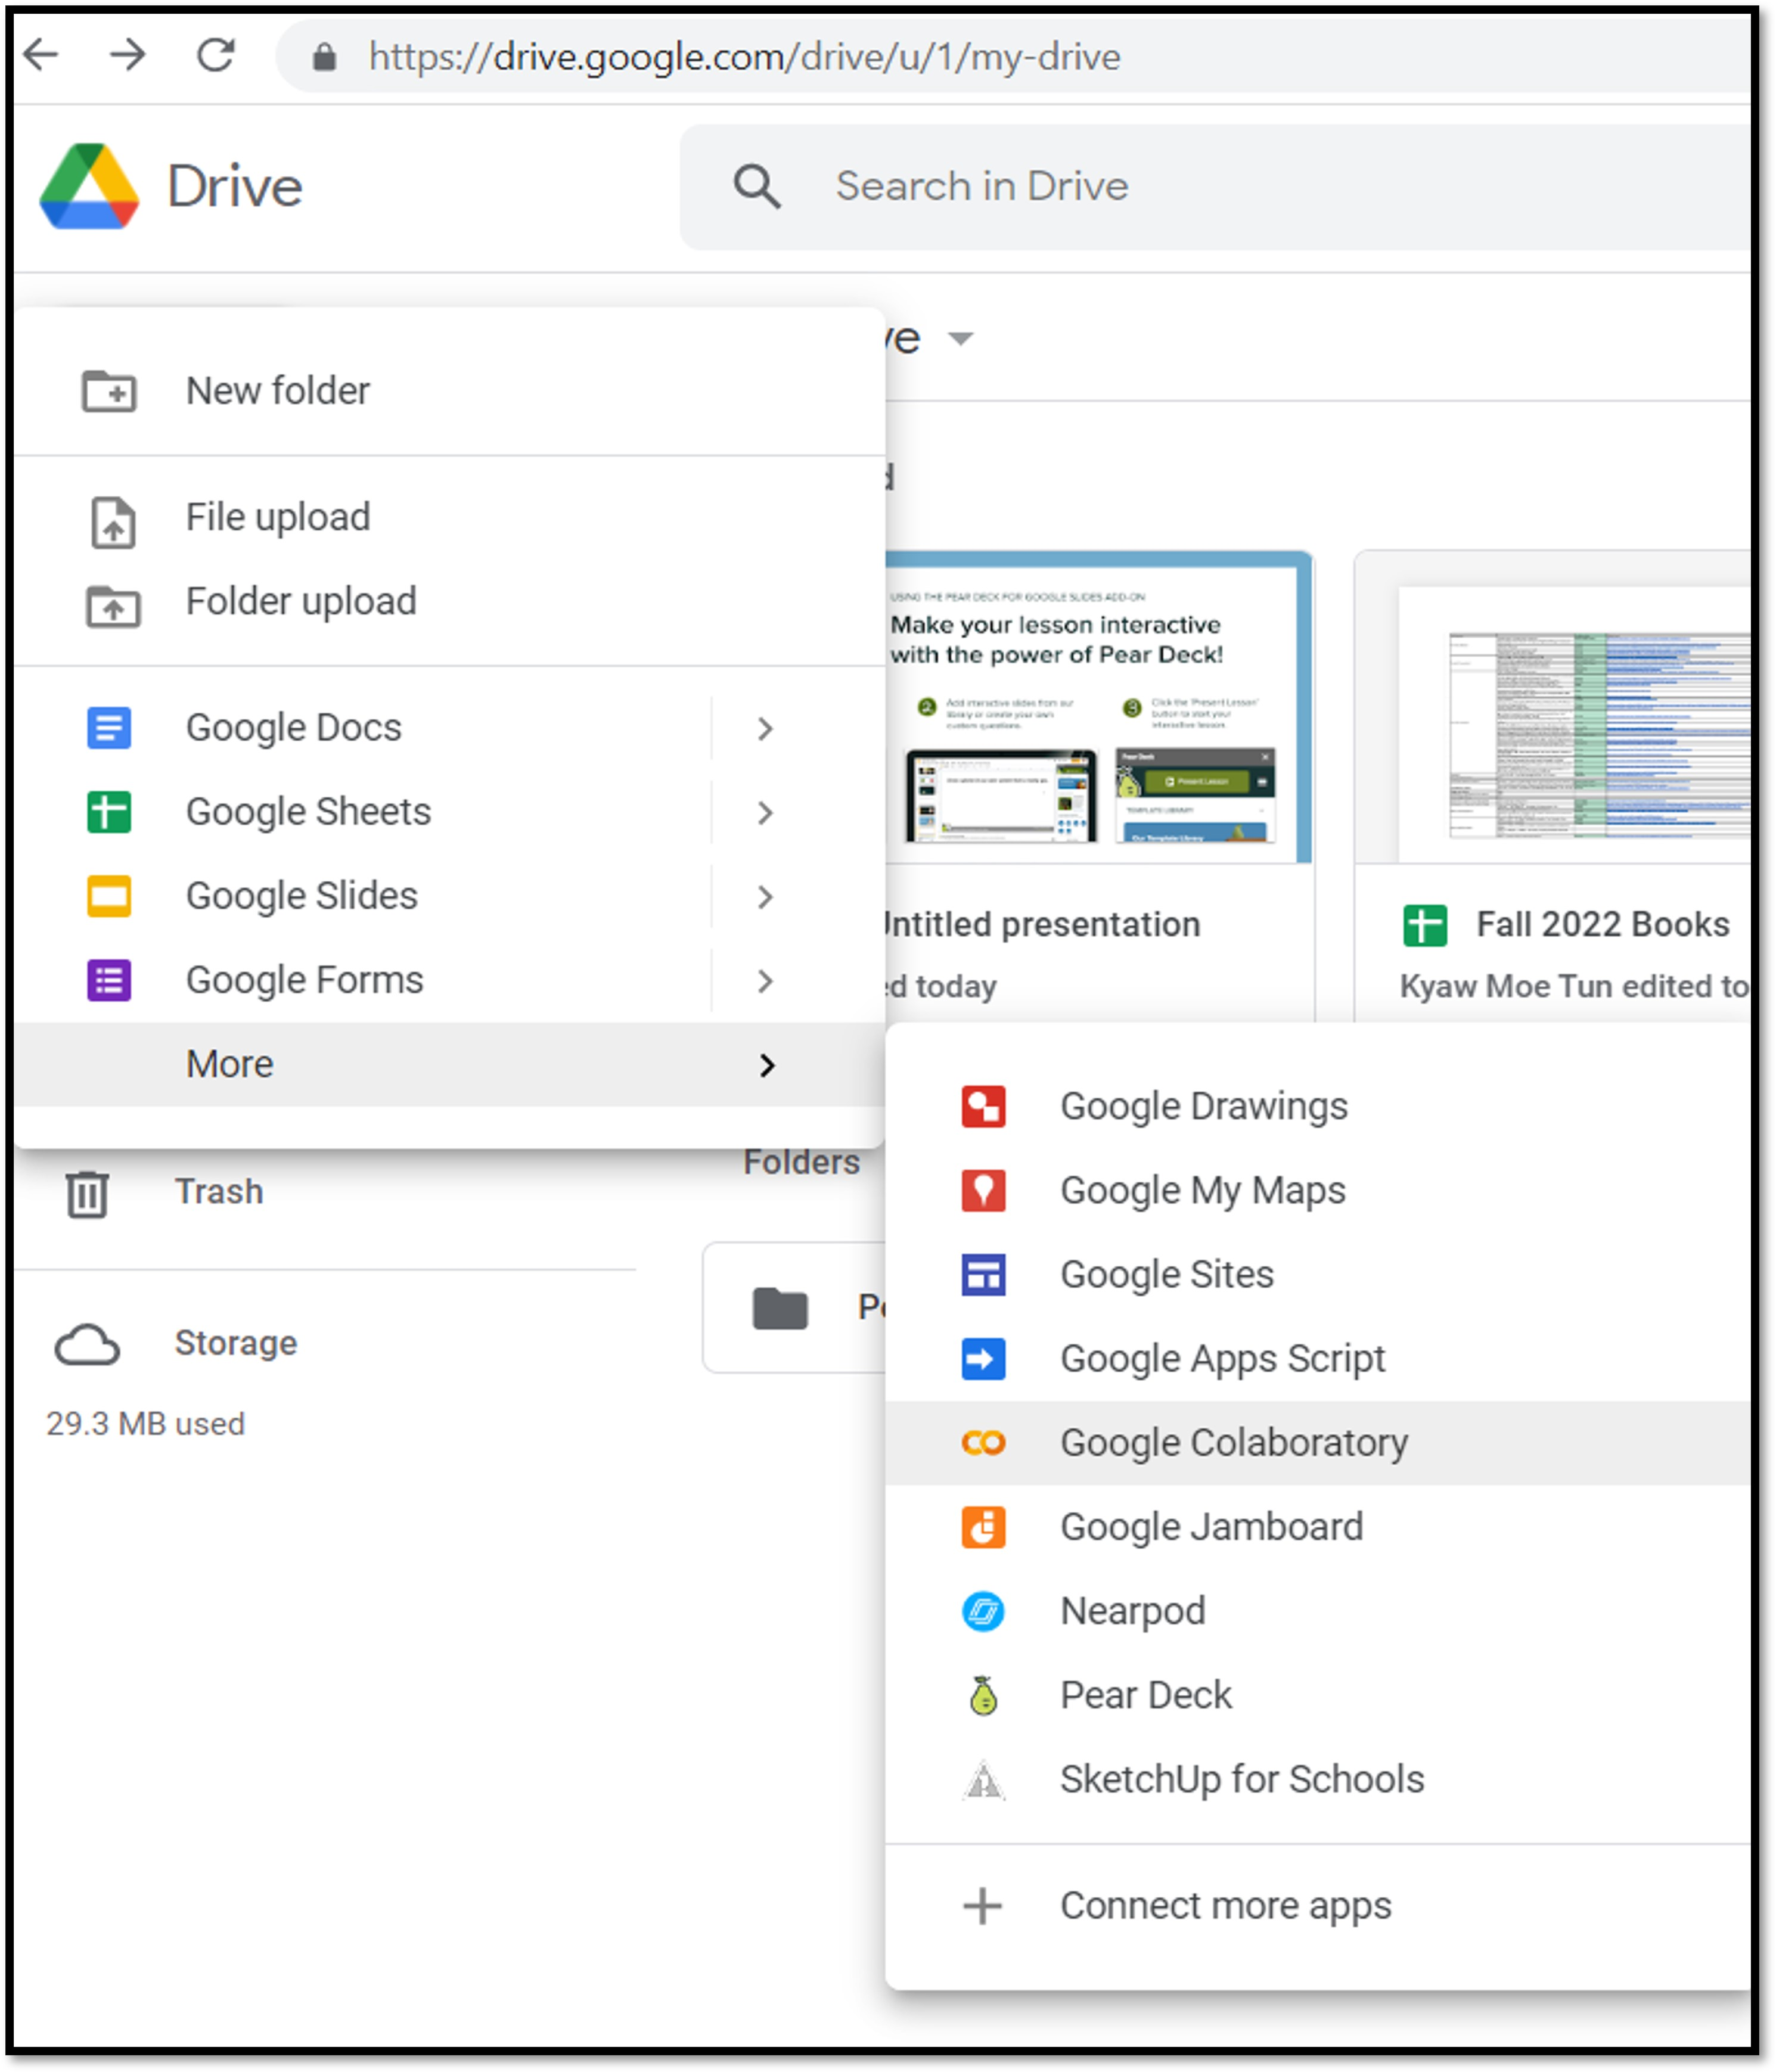
\includegraphics[width=5 cm]{colab1.jpg}
  \caption{Creating a new Colab notebook}
  \label{fig:colab1}
  \end{figure}
   \begin{figure}[!h]
  \centering
  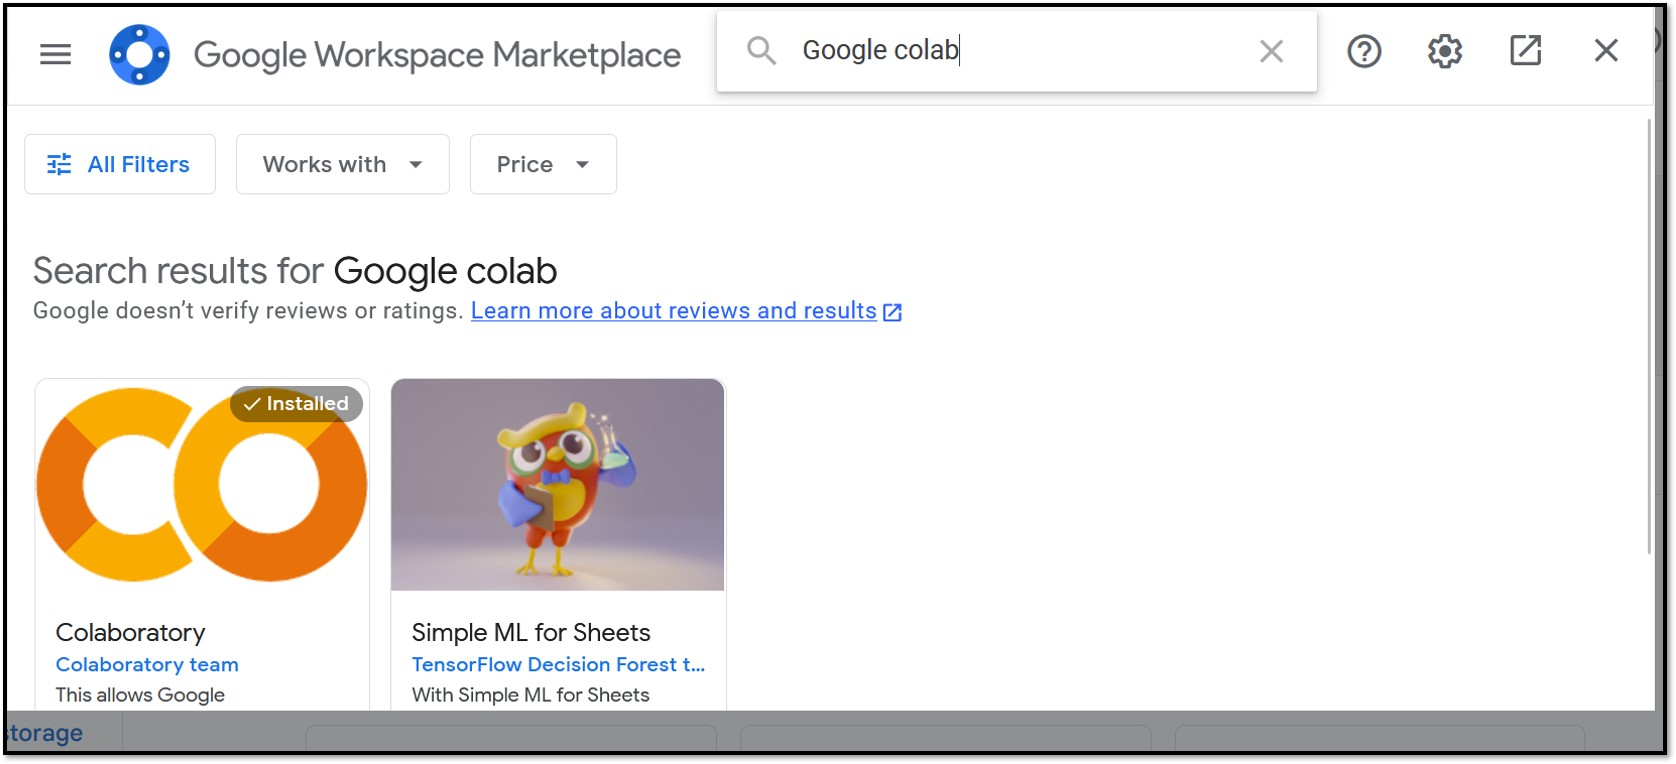
\includegraphics[width=4.5 cm]{colab2.jpg}
  \caption{Connecting to Google Colab App}
  \label{fig:colab2}
  \end{figure}
  \item If you do not find the \emph{Google Colaboratory} in the list, you can click \emph{'Connect more apps'} and search 'Google Colab' in the search bar and add Google Colab to your list as shown in Figure \ref{fig:colab2}.
\end{itemize}
\subsubsection{\textbf{Running a Cell}}
 \begin{itemize}
 \item Make sure the runtime is connected. The notebook shows a green check on the top right corner if it is connected.
 \item Enter your code at the cursor as shown in Figure \ref{fig:colab3}.
 \item To Run cell: press Ctrl + Enter
 \item To Run cell and add new cell below: Alt + Enter
 \item To Run cell and goto cell below: Shift + Enter
 \end{itemize}
 \begin{figure}[h]
  \centering
  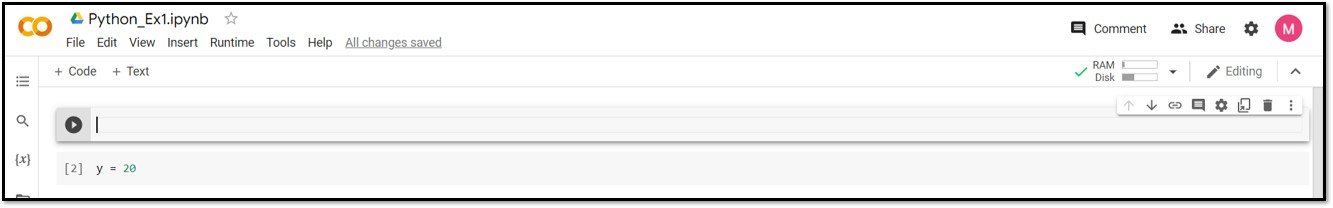
\includegraphics[width=8 cm]{colab3.jpg}
  \caption{Running a cell}
  \label{fig:colab3}
\end{figure}
\newpage
\subsubsection{\textbf{Example Code}}
Figure \ref{fig:import} shows how to read a data file in the Google Colab. Make sure that the files are uploaded into the runtime environment as shown in Figure.
 \begin{figure}[h]
  \centering
  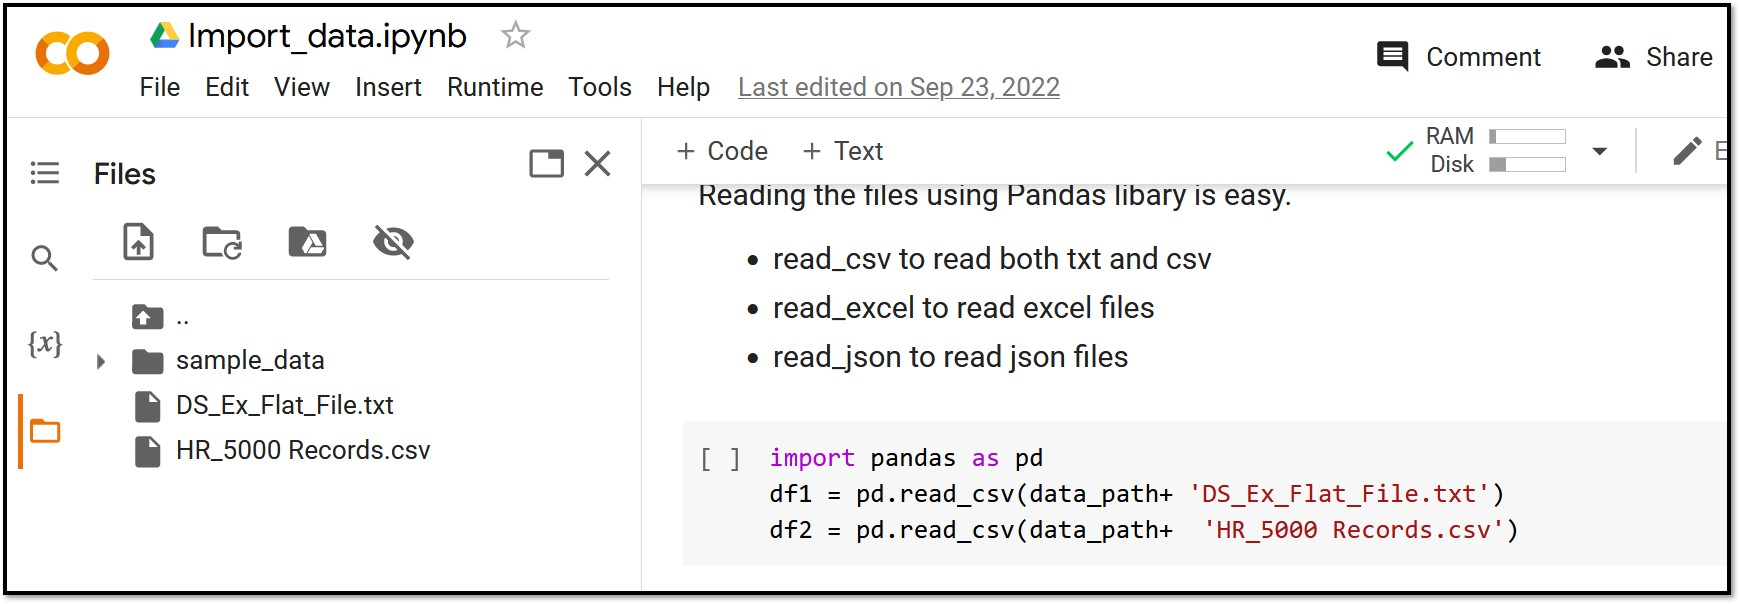
\includegraphics[width=8 cm]{import.jpg}
  \caption{Importing Files}
  \label{fig:import}
\end{figure}
\newpage
\section{Knowledge Test}
\subsection{Supervised or Unsupervised?}
\small{
\begin{questions} %<--- start option fixes number for first question
\question Method to classify if a new patient is having diabetes or not.\\
\begin{oneparchoices}
 \choice  Supervised
 \choice  Unsupervised
\end{oneparchoices}
\question Method to cluster a set of articles into different groups based on similar stories. \\
\begin{oneparchoices}
 \choice  Supervised
 \choice  Unsupervised
\end{oneparchoices}
\question Method to Filter if an email is spam. \\
\begin{oneparchoices}
 \choice  Supervised
 \choice  Unsupervised
\end{oneparchoices}
\question Speech recognition and facial recognition software.\\
\begin{oneparchoices}
 \choice  Supervised
 \choice  Unsupervised
\end{oneparchoices}
\question Segment customer data into groups in marketing environments.\\
\begin{oneparchoices}
 \choice  Supervised
 \choice  Unsupervised
\end{oneparchoices}
\question Detect a fighting event from the CCTV camera.
\begin{oneparchoices}
 \choice  Supervised
 \choice  Unsupervised
\end{oneparchoices}
\end{questions}
}

\subsection{Regression, Classification or Clustering}
\small{
\begin{questions} %<--- start option fixes number for first question
\question Perform initial exploratory analysis on a raw data-set to understand the grouping of data points.\\
\begin{oneparchoices}
 \choice  Regression
 \choice  Classification
 \choice  Clustering
\end{oneparchoices}
\question Method to predict the score of a basketball game. \\
\begin{oneparchoices}
 \choice  Regression
 \choice  Classification
 \choice  Clustering
\end{oneparchoices}
\question You run an online business and you want to predict how many of soft toys will sell over the next month.\\
\begin{oneparchoices}
 \choice  Regression
 \choice  Classification
 \choice  Clustering
\end{oneparchoices}
\question You want to develop an algorithm to check the type of coins (10 baht, 5 baht , 2 or 1 baht).\\
\begin{oneparchoices}
 \choice  Regression
 \choice  Classification
 \choice  Clustering
\end{oneparchoices}
\question Determining whether or not someone will be a defaulter of the loan.\\
\begin{oneparchoices}
 \choice  Regression
 \choice  Classification
 \choice  Clustering
\end{oneparchoices}
\question You run an online shop. You want to group the items sold the most in different seasons.\\
\begin{oneparchoices}
 \choice  Regression
 \choice  Classification
 \choice  Clustering
\end{oneparchoices}
\end{questions}
}
